%!TEX root = ../template.tex
%%%%%%%%%%%%%%%%%%%%%%%%%%%%%%%%%%%%%%%%%%%%%%%%%%%%%%%%%%%%%%%%%%%%
%% chapter3.tex
%% NOVA thesis document file
%%
%% Chapter with a short latex tutorial and examples
%%%%%%%%%%%%%%%%%%%%%%%%%%%%%%%%%%%%%%%%%%%%%%%%%%%%%%%%%%%%%%%%%%%%

\typeout{NT FILE implementation.tex}%

% \makeatletter
% \newcommand{\ntifpkgloaded}{%
%   \@ifpackageloaded%
% }
% \makeatother


\chapter{Implementation}
\label{cha:Implementation}

    % <Given the comprehension of the fundamental concepts let's start the implementation of the system>
    
    % <All of the videos used will be 1920x1080 aspect ratio 16:9 FPS: 60>
    
    % <All of the videos will be from Twitch streams following the structure depicted in \ref{fig:TwitchStreamStructure} and described in \ref{sec:BackInfo}>
    
    % <Each section will represent a milestone and the methodologies used to overcome the challenges encountered.>
    
    % <The first milestone will be the extraction of textual information from the chat of the Twitch stream.>

    We will commence the system implementation upon grasping the fundamental concepts related to video analysis and image processing techniques. We will provide a detailed explanation of our developed work, elucidating the high-level characteristics extractable from the videogame stream and demonstrating how this information can be accessed in real time. All videos will adhere to 1920x1080 resolution, 16:9 aspect ratio, and 60 FPS. Content will be sourced from \href{https://www.twitch.tv/}{Twitch} streams, following the structure outlined in Figure \ref{fig:TwitchStreamStructure} and detailed in Section \ref{sec:BackInfo}. Milestones will guide our progress, with each section tackling challenges encountered and methodologies employed.
    
    The initial milestone focuses on extracting the viewers interactions from \href{https://www.twitch.tv/}{Twitch} stream chat.

\section{Twitch chat}

    % <The video broadcast structure on the Twitch platform consists of five essential components, as described in \ref{sec:BackInfo}>. One of them is the chat, where the streamer and viewers can interact with each other>

    % <This component is crucial to identify important moments in the gameplay. The interactions in the chat can be interpreted as descriptions of the important moments. For example, when multiple viewers use the chat to congratulate the streamer of a good play or a good game, it translates to the possibility that the previous gameplay streamed was of great importance.>
    
    % <This component is then sub-composed by a header at the top with the text STREAM CHAT, an input box at the bottom where the viewer of the stream can write to the chat, and between these, there are the interactions between the viewers and the streamer. These interactions can also include emotes, small animations that are sometimes restricted to the stream watched. \cite{TwitchChatBasics}>

    The Twitch platform's video broadcast structure comprises five essential components, detailed in \ref{sec:BackInfo}. Among these, the chat function serves as a vital tool for identifying significant moments in gameplay, enabling interaction between streamers and viewers. Chat interactions often serve as descriptors of pivotal moments; for instance, multiple congratulatory messages may indicate a noteworthy gameplay segment.
    
    The chat component can be further segmented into a header labeled 'STREAM CHAT,' an input box for viewer participation, and the ongoing interactions between viewers and the streamer, as depicted in the article \cite{TwitchChatBasics}. These interactions may also feature emotes (small animations) often specific to the watched stream.
    
    % <Describe the composition of the messages: timestamp (username): message>

    % <Figure depicting the chat and its subcomponents>

    % MAYBE SET IN THE INTERACTION SEPARATION
    Every interaction within the chat can be segmented into three key components, as depicted in Figure \ref{fig:TwitchStreamChatSettings}: the timestamp denoting the system time of the interaction, the username of the participant, and the message content.

    \begin{figure}[htbp]
        \centering
        \fboxsep=0pt\fboxrule=0.5pt
        \fbox{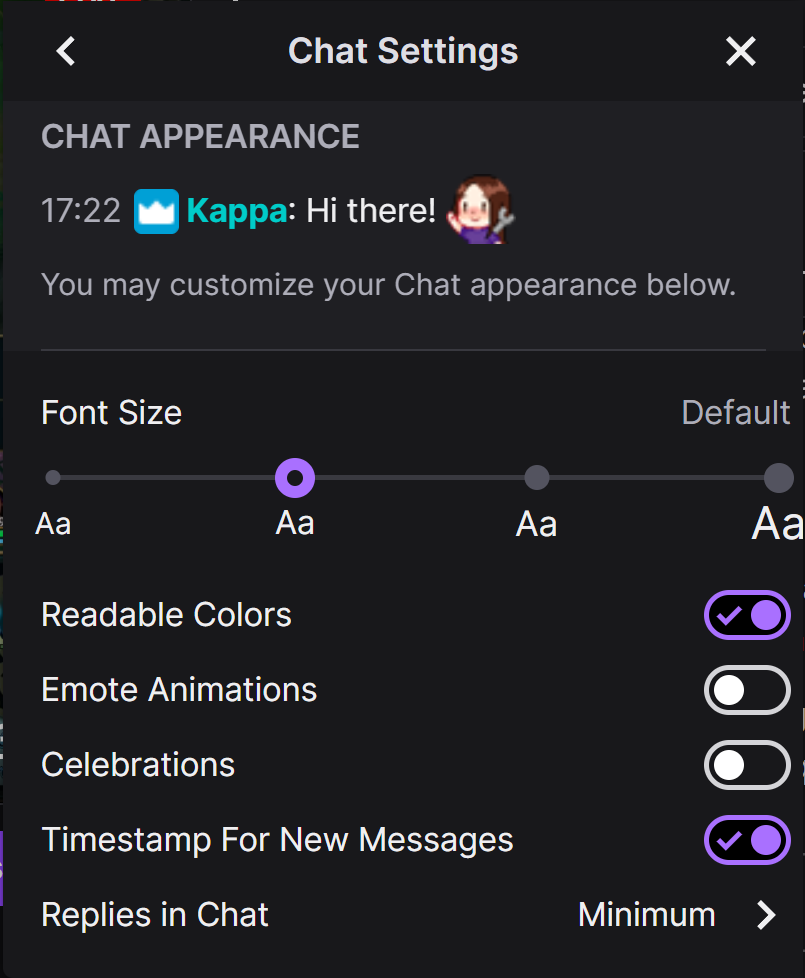
\includegraphics[width=0.8\linewidth]{Chapters/Figures/InteractionComponents.png}}%
        \caption{Composition of the interactions within the Twitch chat (screenshot of the Appearance Settings)}
        \label{fig:TwitchStreamChatSettings}
    \end{figure}

    % <The chat is not always being updated seeing that not every game moment is worthy of an interaction. To only extract the interactions of the chat when there is a new interaction added it is necessary to identify when there is a chat update.>

    % <To identify when the chat is updated with new interactions, an algorithm was developed to compare two consecutive frames of the stream. The methodology used is based on the binary operation XOR \cite{BitwiseOperationsOpenCV}. When applied the operation between these two consecutive frames the differences are highlighted and the similarities are cancelled. This operation results in a matrix of pixels that are highlighted on the pixels where there are differences.>

    The ongoing interactions are not always being updated seeing that not every game moment is worthy of an interaction, so the viewers do not output messages to the chat. To only extract the interactions of the chat when there is a new interaction added it is necessary to identify when there is a chat update. For that challenge was developed an algorithm to compare two consecutive frames of the stream, based on the binary operation XOR \cite{BitwiseOperationsOpenCV}. The operation between these two successive frames highlights the differences and eliminates the similarities. This process generates a matrix of pixels, having differences highlighted in the values of the three RGB channels.    

    % < However the resulting matrix is not always completely darkened or completely highlighted, due to the possibility of the emotes present in the interactions. The movement of these emotes can be perceived as differences in the \gls{XOR} operation, as depicted in Figure X.X. So it is necessary to establish a threshold to differentiate the chat update from the occasional movement of the emotes.>

    However, because emotes may be included in the interactions, the resulting matrix can occasionally not be entirely highlighted or darkened. As seen in FIGURE X.X, these emotes' movements can be perceived as variations in the \gls{XOR} operation. Therefore, a threshold needs to be set to distinguish the chat update from the sporadic emotive movement.

    <Images: Original two frames for each case (one when there is no change and when there is)>

    

    

    

    